\documentclass[11pt,oneside]{article}
\usepackage[T1]{fontenc}
\usepackage[utf8]{inputenc}
%\DeclareUnicodeCharacter{00A0}{ }
\usepackage[adobe-utopia]{mathdesign}

\usepackage{amsmath}
\usepackage[francais]{babel}
\usepackage[dvips]{graphicx}
%\usepackage{here}
\usepackage{framed}
\usepackage[normalem]{ulem}
\usepackage{fancyhdr}
\usepackage{titlesec}
\usepackage{vmargin}

\usepackage{amsmath}
\usepackage{ifthen}
\usepackage{multirow}
\usepackage{multicol} % Portions de texte en colonnes

%\usepackage{xltxtra} % Logo XeLaTeX
%\usepackage{pst-solides3d}
\usepackage{color}
%\usepackage{colortbl}
\usepackage{titletoc} % Pour la mise en forme de la table des matières

%\usepackage[crop=off]{auto-pst-pdf}
%\usepackage{bclogo}


%\usepackage{longtable}
%\usepackage{flafter}%floatants après la référence
%\usepackage{pst-solides3d}
%\usepackage{pstricks}
%\usepackage{minitoc}
%\setcounter{minitocdepth}{4}
%\usepackage{draftcopy}% "Brouillon"
%\usepackage{floatflt}
%\usepackage{psfrag}
%\usepackage{listings} % Permet d'insérer du code de programmation
%\usepackage{lmodern}
%\usepackage[adobe-utopia,uppercase=upright,greeklowercase=upright]{mathdesign}
%\usepackage{minionpro}
%\usepackage{pifont}
%\usepackage{amssymb}
%\usepackage[francais]{varioref}

\setmarginsrb{1.5cm}{1cm}{1cm}{1.5cm}{1cm}{1cm}{1cm}{1cm}

\definecolor{gris25}{gray}{0.75}
\definecolor{bleu}{RGB}{18,33,98}
\definecolor{bleuf}{RGB}{42,94,171}
\definecolor{bleuc}{RGB}{231,239,247}
\definecolor{rougef}{RGB}{185,18,27}
\definecolor{rougec}{RGB}{255,230,231}
\definecolor{vertf}{RGB}{103,126,82}
\definecolor{vertc}{RGB}{220,255,191}
\definecolor{violetf}{RGB}{112,48,160}
\definecolor{violetc}{RGB}{230,224,236}
\definecolor{jaunec}{RGB}{220,255,191}
\usepackage[raccourcis]{FAST}
\usepackage[%
    pdftitle={Conception -- Liaisons encastrement},
    pdfauthor={Xavier Pessoles},
    colorlinks=true,
    linkcolor=blue,
    citecolor=magenta]{hyperref}
\usepackage{schemabloc}



% \makeatletter \let\ps@plain\ps@empty \makeatother
%% DEBUT DU DOCUMENT
%% =================
\sloppy
\hyphenpenalty 10000

\newcommand{\Pointilles}[1][3]{%
\multido{}{#1}{\makebox[\linewidth]{\dotfill}\\[\parskip]
}}


\colorlet{shadecolor}{orange!15}

\newtheorem{theorem}{Theorem}


\begin{document}


\newboolean{prof}
\setboolean{prof}{true}
%------------- En tetes et Pieds de Pages ------------
\pagestyle{fancy}
\renewcommand{\headrulewidth}{0pt}

\fancyhead{}
\fancyhead[L]{%
\noindent\noindent\begin{minipage}[c]{2.6cm}
%Lycée Rouvière PTSI

\includegraphics[width=2cm]{png/logo_ptsi.png}%
\end{minipage}
}

\fancyhead[C]{\rule{12cm}{.5pt}}

\fancyhead[R]{%
\noindent\begin{minipage}[c]{3cm}
\begin{flushright}
\footnotesize{\textit{\textsf{Sciences Industrielles\\ pour l'Ingénieur}}}%
\end{flushright}
\end{minipage}
}

\renewcommand{\footrulewidth}{0.2pt}

\fancyfoot[C]{\footnotesize{\bfseries \thepage}}
\fancyfoot[L]{\footnotesize{2012 -- 2013} \\ X. \textsc{Pessoles}}
\ifthenelse{\boolean{prof}}{%
\fancyfoot[R]{\footnotesize{Cours -- CI : Conception -- P}}
}{%
\fancyfoot[R]{\footnotesize{Cours -- CI : Conception}}
}



\begin{center}
 \huge\textsc{CI 4 -- Conception : Conception des mécanismes}
\end{center}

\begin{center}
 \LARGE\textsc{Chapitre 2 -- Conception des liaisons encastrement}
\end{center}

\vspace{.5cm}

\begin{center}
\begin{tabular}{ccc}
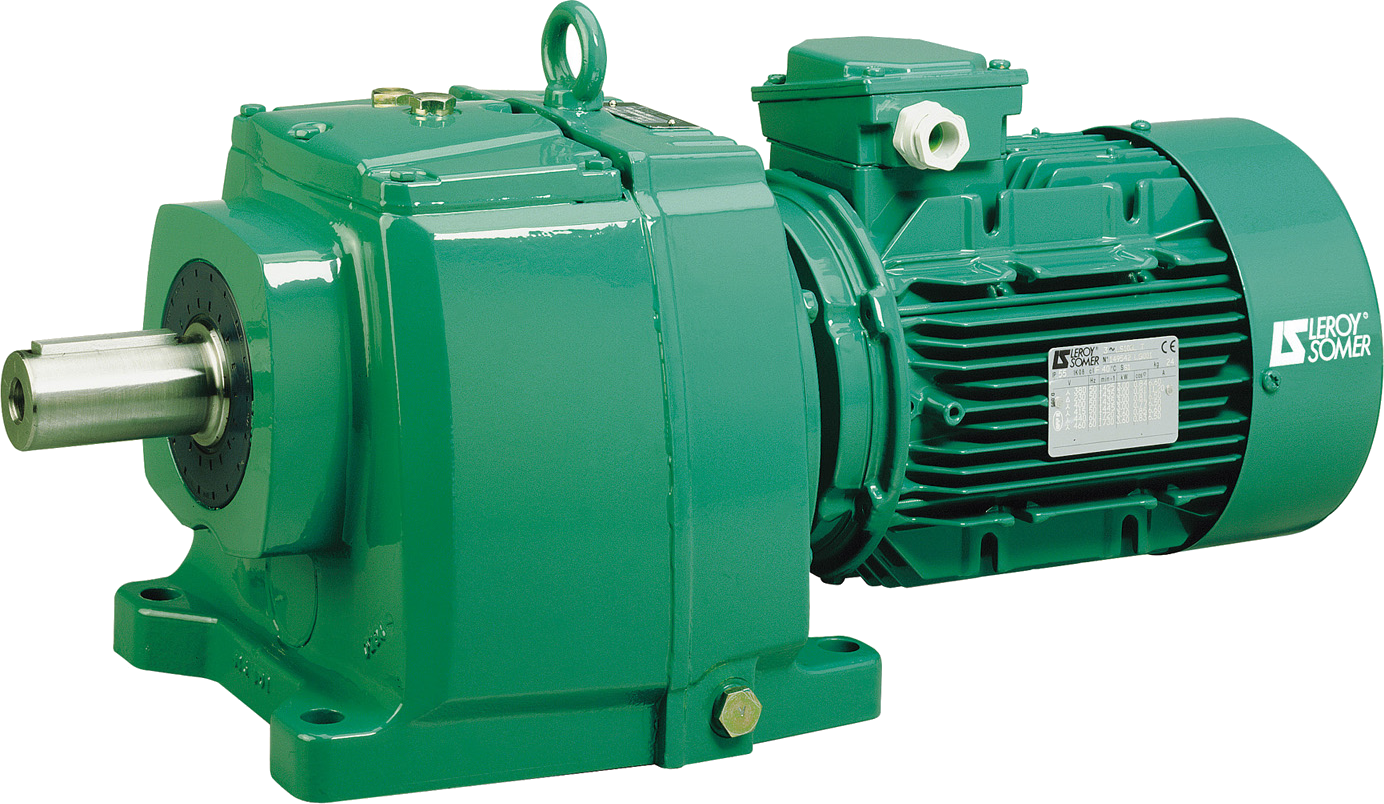
\includegraphics[height=3cm]{png/motored1} &
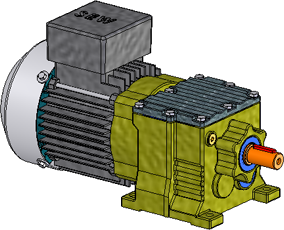
\includegraphics[height=3cm]{png/motored2} &
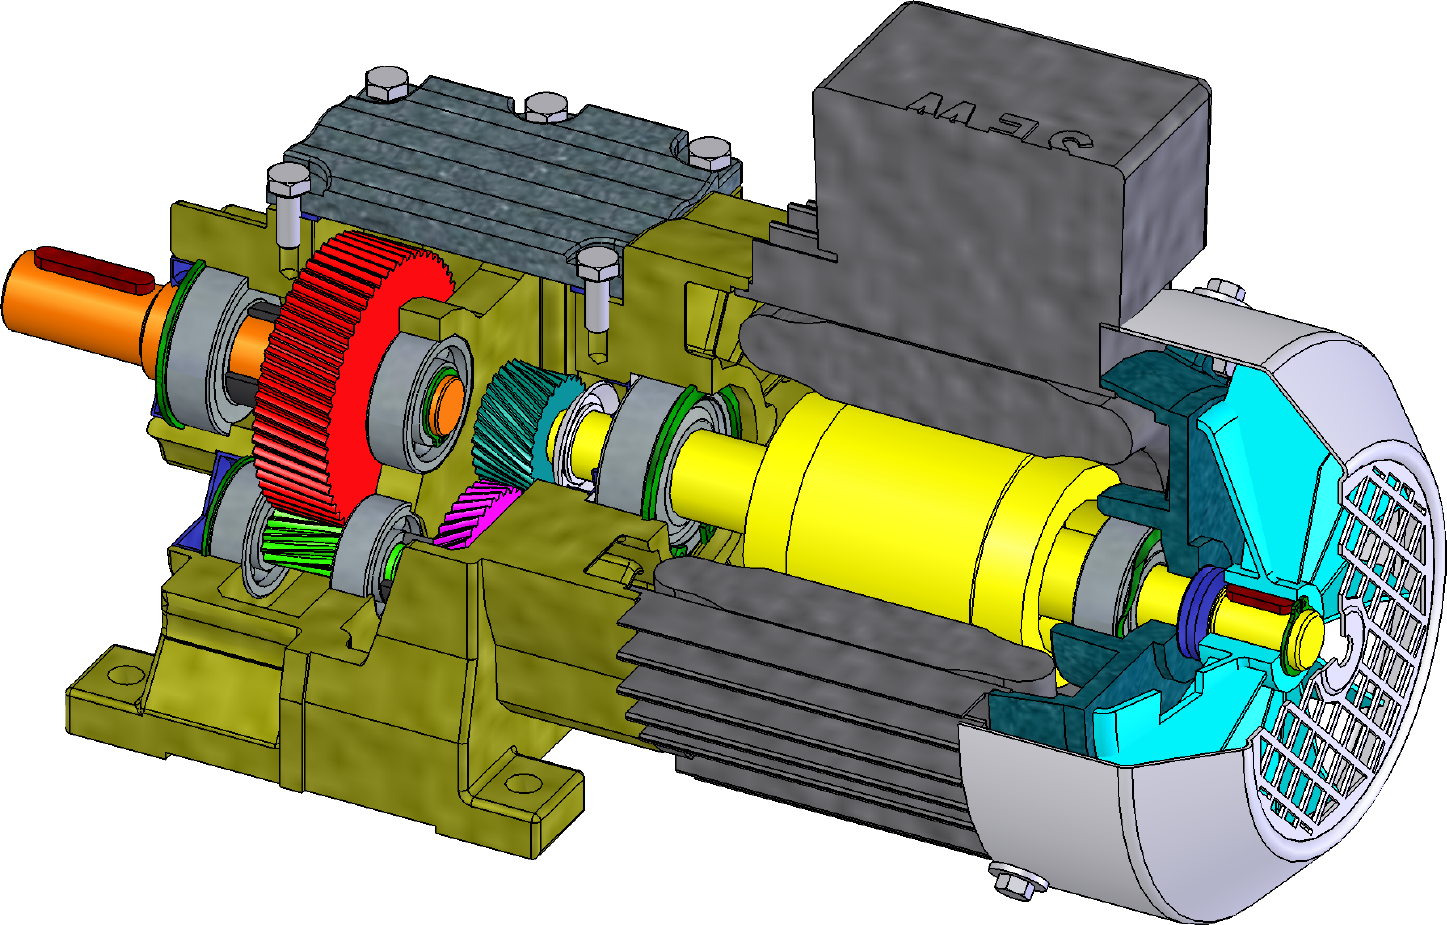
\includegraphics[height=3cm]{png/motored3} \\
\textit{Motoréducteur Leroy Somer \cite{ls}} & \textit{Motoréducteur SEW}&\textit{Écorché}\\
\end{tabular}
\end{center}

La liaison encastrement est au c\oe{}ur de la conception des systèmes mécanique. D'une part, tous les systèmes comprennent un bâti composé de pièces fixes les unes par rapport aux autres. D'autre part, les classes d'équivalences cinématiques participant à la transmission ou à la transformation de puissance, sont elles-mêmes constituées de pièces fixes les unes par rapport aux autres. 

Ces liaisons encastrement peuvent être démontables, permettant ainsi d'assurer la maintenance d'une pièce ou d'une autre. Elles peuvent être aussi permanentes (ou non démontables). Dans ce cas, il faut faire appel à des procédés d'assemblage plus ou moins difficiles à mettre en \oe{}uvre. 

Parmi la multitude de solutions technologiques qui peuvent se présenter, il s'agit d'abord de choisir de façon méthodique celle à même de répondre au cahier des charges puis enfin de savoir la représenter en vu de concevoir un mécanisme.

\begin{prob}
\textsc{Problématique :}
\begin{itemize}
\item Décrire ou choisir les solutions technologiques réalisant un encastrement.
\item Représenter une solution complète avec les conditions de fonctionnement.
\end{itemize}
\end{prob}

\begin{savoir}
\textsc{Savoirs :}
\begin{itemize}
\item Définir et caractériser une fonction d'assemblage.
\item Principes d'immobilisation par obstacle(s) ou par adhérence.
\item Familles de solutions, critères de choix, solutions techniques par plan prépondérant, cylindre prépondérant, cône prépondérant.
\item Conditions d'utilisations et calculs relatifs à la transmission d'un couple ou d'un glisseur.
\end{itemize}
\end{savoir}

\newpage 

\setlength{\parskip}{0ex plus 0.2ex minus 0ex}
 \renewcommand{\contentsname}{}
 \renewcommand{\baselinestretch}{1}

\tableofcontents

 \renewcommand{\baselinestretch}{1.2}
\setlength{\parskip}{2ex plus 0.5ex minus 0.2ex}

% \vspace{1cm}
\textit{Ce document est en évolution permanente. Merci de signaler toutes
erreurs ou coquilles.}

\newpage

\section*{Introduction}

Dans le cas général, la fonction \textbf{réaliser une liaison encastrement démontable} peut se décomposer selon le FAST qui suit (Liste non exhaustive des solutions). 
Dans le cours qui suit, nous allons nous attacher à décrire quelques sont les solutions technologiques qui peuvent permette de réaliser ces fonctions principales.

\FASTInterligne=.2cm %Nouvel interligne
\begin{FAST}{Réaliser une liaison encastrement démontable}
\FASTFT{FP1 -- Réaliser la mise en position entre pièces (MIP)}{%
	\FASTFT{FP11 -- Assurer une liaison prépondérante}{%
		\FASTST{Appui plan}
		\FASTDecalageOuHorizontal=0pt
		\FASTST[ou]{Cylindre long (pivot glissant)}
	\FASTDecalageOuHorizontal=0pt
		\FASTST[ou]{Cône (pivot)}}
	\FASTFT{FP12 -- Assurer une liaison secondaire}{
		\FASTST{Cylindre court (Sphère -- cylindre)}
		\FASTDecalageOuHorizontal=0pt
		\FASTST[ou]{Contact ponctuel}}}
\FASTFT{FP2 -- Réaliser le maintien en position entre pièces (MAP)}{
		\FASTST{Éléments filetés}
		\FASTDecalageOuHorizontal=0pt
		\FASTST[ou]{Soudage}
		\FASTDecalageOuHorizontal=0pt
		\FASTST[ou]{Colles}}
\FASTFT{FP3 -- Transmettre la puissance}{
		\FASTST{Pions}
		\FASTDecalageOuHorizontal=0pt
		\FASTST[ou]{Clavette (parallèles, disque...)}
		\FASTDecalageOuHorizontal=0pt
		\FASTST[ou]{Cannelures}}
\FASTFT{FP4 -- Assurer l'étanchéité}{
		\FASTST{Joint torique, joint papier...}
		\FASTDecalageOuHorizontal=0pt
		\FASTST[ou]{Colles}}
\FASTFT{FP5 -- Assurer la fiabilité}{
		\FASTST{Freinage des écrous : rondelles éventail, écrou nylstop, ...}}
\end{FAST}
\FASTReset %Remise à zéro


\section{Réaliser la mise en position entre pièces}
\subsection{Architectures isostatiques des liaisons encastrement}
Réaliser une liaison encastrement revient tout d'abord à créer une mise en position. Il s'agit donc de supprimer les 6 degrés de liberté existants entre deux pièces. \'A toutes les combinaisons de 6 liaisons sphère--plan permettant d'arriver à cette fin correspondent autant d'architectures de conceptions de produits.



%\vspace{.5cm}


\subsection{Liaison avec appui plan prépondérant}
Les liaisons encastrements à appui plans prépondérants sont souvent utilisés entre le carter d'un mécanisme et des pièces environnantes.

\'A partir d'un appui plan, 3 degrés de liberté restent à supprimer. Une des solutions peut être d'utiliser la combinaison d'une liaison sphère-cylindre et d'une liaison sphère plan (voir ci-dessous). Cette solution est souvent utilisée lorsqu'il s'agit de mettre en position un arbre par un flasque (arbre débouchant) ou par un chapeau (arbre non débouchant).


\noindent\begin{minipage}[c]{.45\linewidth}
\begin{center}
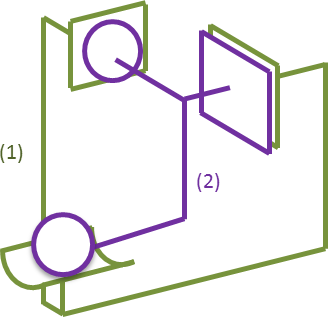
\includegraphics[height=4cm]{png/archi2}

\textbf{Architecture à appui plan prépondérant}
\end{center}
\end{minipage}\hfill
\noindent\begin{minipage}[c]{.45\linewidth}
\begin{center}
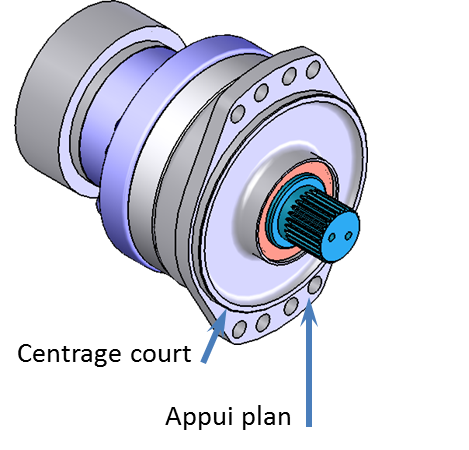
\includegraphics[width=.8\textwidth]{png/poclain_2}

\textbf{Moteur pneumatique Poclain \cite{poclain} -- Surfaces fonctionnelles d'assemblage}
\end{center}
\end{minipage}

\vspace{.5cm}

Dans le cas ci-dessus, la liaison sphère -- cylindre est réalisée par un centrage court, c'est à dire un épaulement sur chacune des deux pièces. \'A ce stade, 5 degrés de liberté sont supprimés. La liaison équivalente entre les deux pièces est alors une liaison pivot. 
Il reste alors à supprimer la rotation relative entre les deux pièces. Dans le cas où il n'y a pas besoin d'indexer une pièce par rapport à l'autre et qu'il ne faut transmettre aucun effort, le sixième degré de liberté peut être supprimé par des vis. Cependant, on évitera cette solution. En effet, \textbf{les vis n'ont pas pour but d'assurer une mise en position}. 

Pour supprimer le dernier degré de liberté, on peut alors utiliser \textbf{des goupilles}. Elles 
peuvent être de géométries diverses : 

\vspace{.25cm}
\noindent \begin{minipage}[c]{.25\linewidth}
\begin{itemize}
\item goupilles cylindriques;
\item goupilles coniques;
\item goupilles élastiques;
\item goupilles fendues.
\end{itemize}
\end{minipage} \hfill
\begin{minipage}[c]{.7\linewidth}
\begin{center}
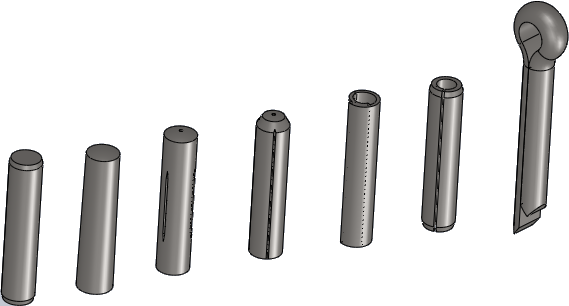
\includegraphics[width=.6\textwidth]{png/goupilles}
\end{center}
\end{minipage} 
\vspace{.25cm}

Une traduction d'une mise en position avec appui-plan prépondérant, centrage court et goupille d'indexage est présentée-ci dessous. 

\vspace{.5cm}
\noindent\begin{minipage}[c]{.45\linewidth}
\begin{center}
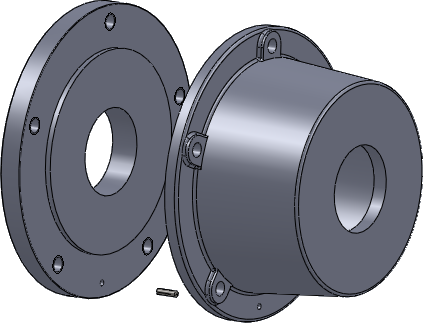
\includegraphics[height=5cm]{png/PlanPrep_1}
\end{center}
\end{minipage}\hfill
\noindent\begin{minipage}[c]{.45\linewidth}
\begin{center}
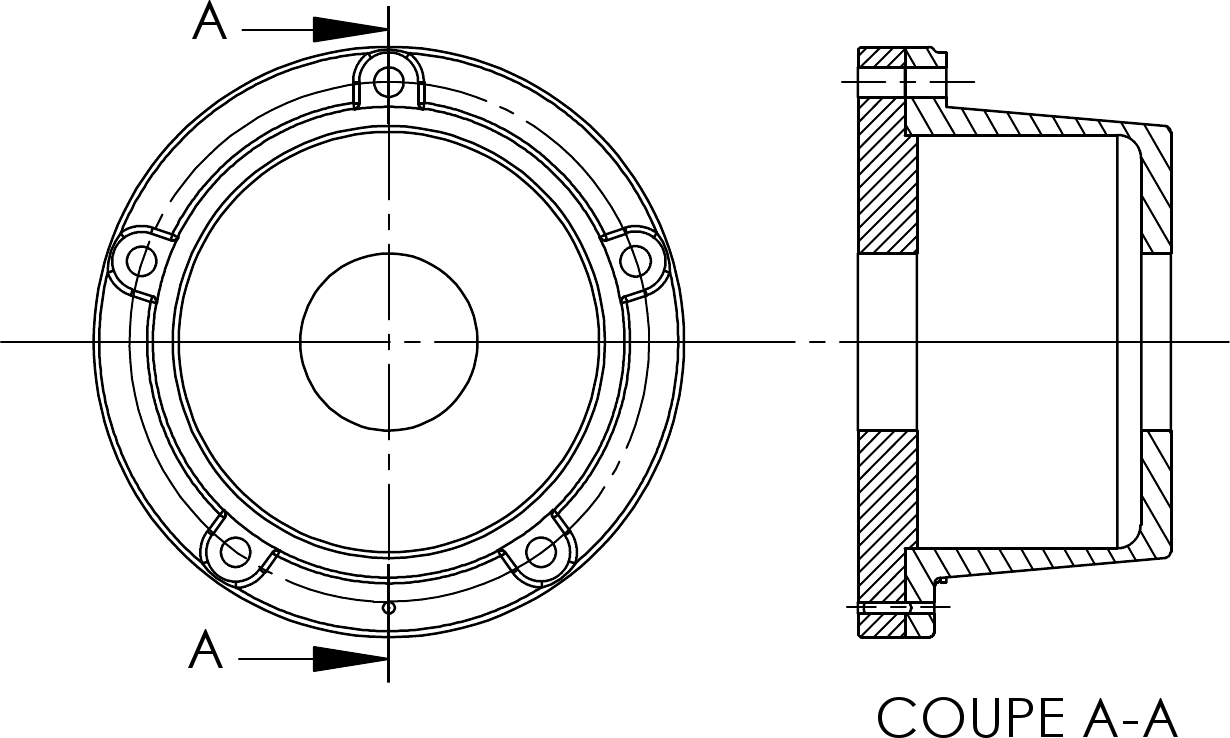
\includegraphics[height=5cm]{png/PlanPrep_2}
\end{center}
\end{minipage}

\vspace{.5cm}

En remplacement au centrage court, une solution peut être d'utiliser une goupille pour réaliser ce centrage. Reste alors un degrés de liberté qui est supprimé par un locating. Suivant les cas, ce locating peut être réalisée par une pièce avec une forme oblongue (comme ci-dessous) ou par un pion et une trou de forme oblong dans une des pièces. 

\vspace{.5cm}

\noindent\begin{minipage}[c]{.3\linewidth}
\begin{center}
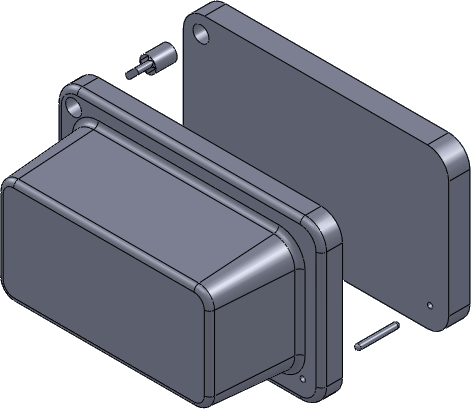
\includegraphics[width=.9\textwidth]{png/PlanPrep_3}
\end{center}
\end{minipage}\hfill
\noindent\begin{minipage}[c]{.65\linewidth}
\begin{center}
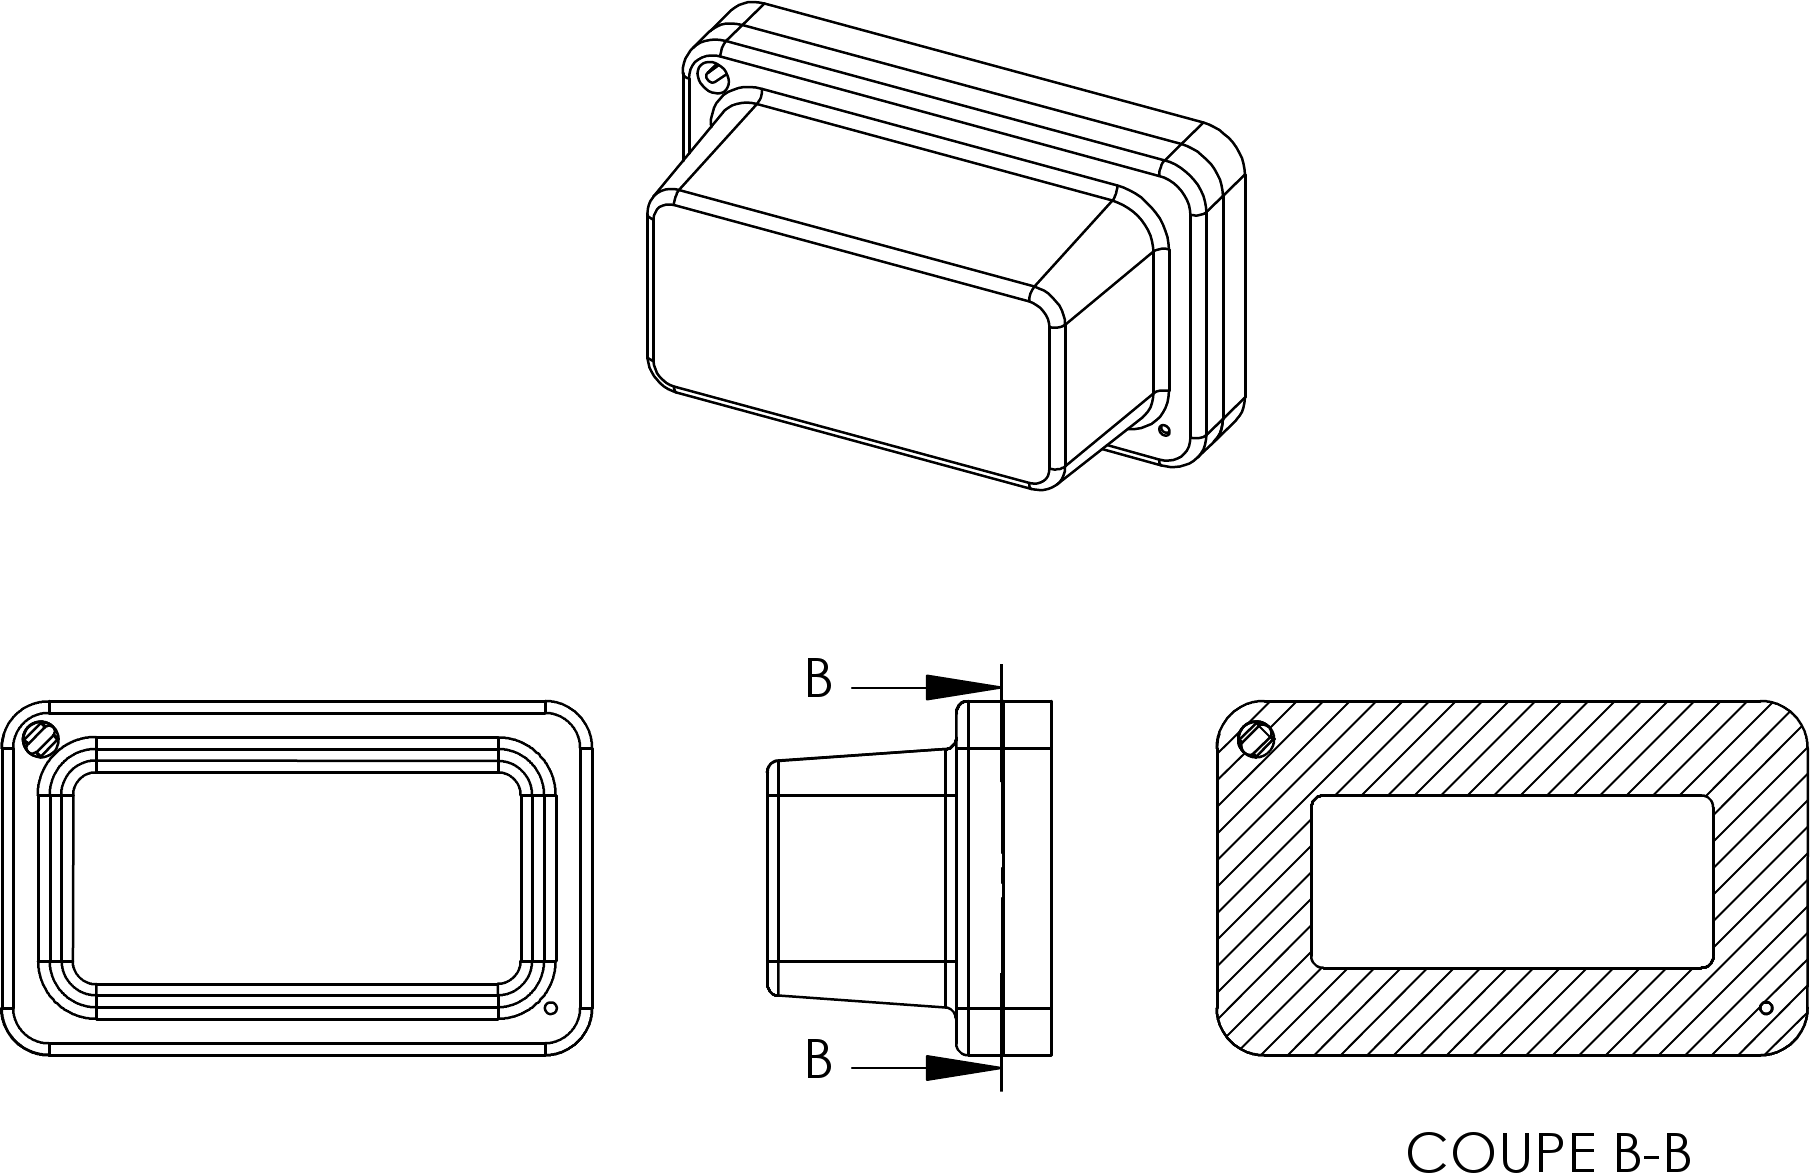
\includegraphics[width=\textwidth]{png/PlanPrep_4}
\end{center}
\end{minipage}

\vspace{.5cm}

\noindent\begin{minipage}[c]{.3\linewidth}
\begin{center}
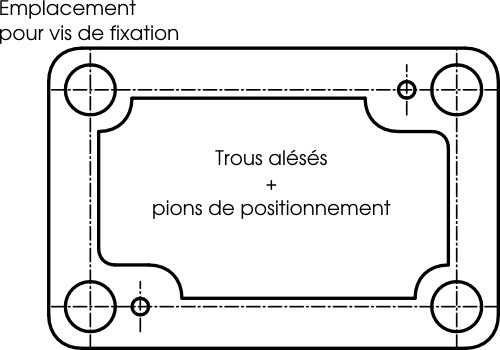
\includegraphics[width=.9\textwidth]{png/Fig19}
\end{center}
\end{minipage}\hfill
\noindent\begin{minipage}[c]{.65\linewidth}
\begin{center}
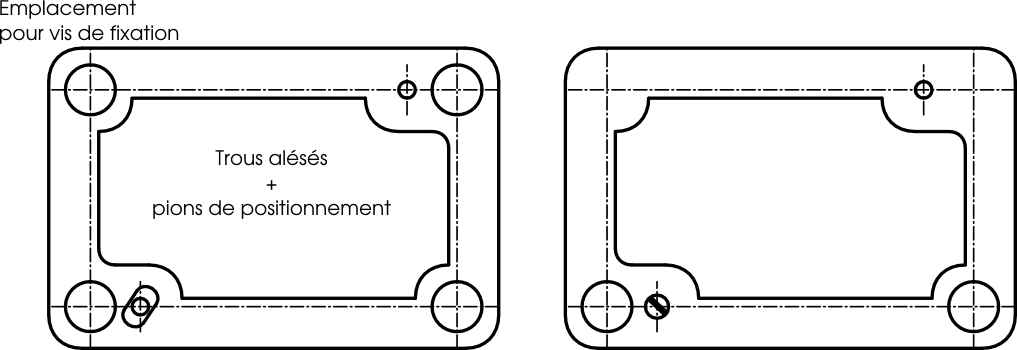
\includegraphics[width=\textwidth]{png/Fig21}
\end{center}
\end{minipage}

\vspace{.5cm}

\begin{center}
\begin{minipage}[c]{.3\linewidth}
\begin{center}
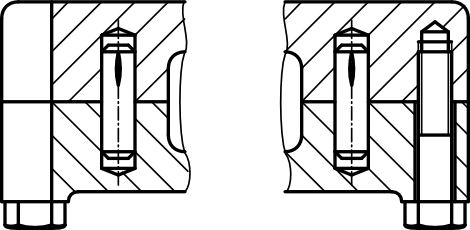
\includegraphics[width=.9\textwidth]{png/Fig18}
\end{center}
\end{minipage}
\end{center}

\subsection{Liaison avec cylindre long prépondérant}

Cette architecture de liaison est très utilisée dans le but de mettre en position des pignons ou des poulies sur des arbres. 


\noindent\begin{minipage}[c]{.45\linewidth}
\begin{center}
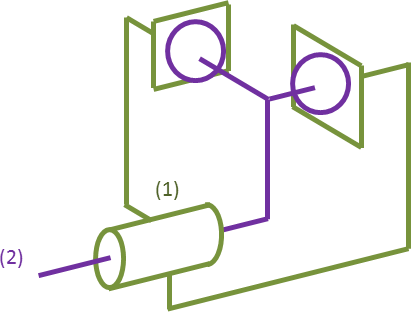
\includegraphics[height=4cm]{png/archi1}

\textbf{Architecture à cylindre long prépondérant}
\end{center}
\end{minipage}\hfill
\noindent\begin{minipage}[c]{.45\linewidth}
\begin{center}
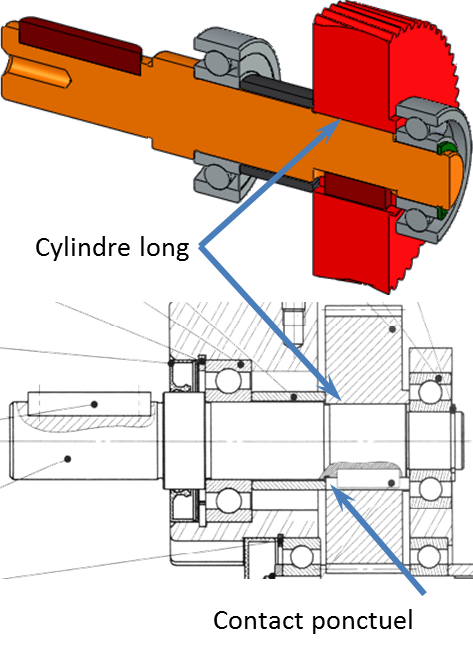
\includegraphics[width=.8\textwidth]{png/sew_1}

\textbf{Motoréducteur SEW \cite{sew} -- Montage d'une poulie}
\end{center}
\end{minipage}

\vspace{.5cm}

Comme son nom l'indique, cette liaison est basée sur la mise en contact de deux cylindres sur une longueur relativement importante. 

Dans la mesure du possible l'arrêt en translation sera réalisé par un \textbf{épaulement}. Cette solution est en effet relativement à réaliser sur un arbre et offre une bonne robustesse. 

Dans d'autres cas, cet arrêt pourra être réalisé par une entretoise ou encore par un anneau élastique (circlips). 

Enfin, le blocage en rotation peut être assuré par adhérence, par un ajustement serré (le montage est alors obtenu grâce à une presse ou par frettage). Lorsque qu'il existe un couple à transmettre entre les pièces, on peut alors utiliser des arrêts avec des goupilles (entre cuir et chair), des clavettes (parallèles ou disque) voire des cannelures. Ces dispositions permettant d'assurer la transmission du couple sont présentées ultérieurement. 

\subsection{Liaison avec cône prépondérant}
\begin{minipage}[c]{.7\linewidth}
Les liaisons utilisant des cônes sont par exemple utilisés dans les systèmes d'attachement des machines outils, entre les porte outils et les outils. La liaison cône -- cône permet de réaliser une liaison pivot. Il reste alors à immobiliser les solides en rotations. Pour cela on utilise un "lardon". 
\end{minipage}\hfill
\begin{minipage}[c]{.25\linewidth}
\begin{center}
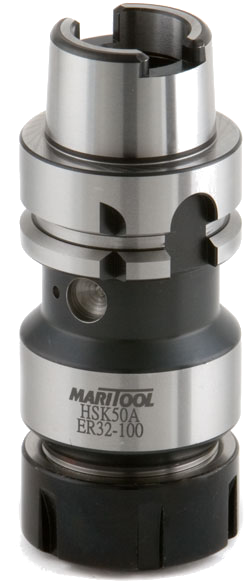
\includegraphics[height=4cm]{png/hsk}

\textit{Attachement KSK \cite{attachements_2}}
\end{center}
\end{minipage}

\vspace{.5cm}

\noindent\begin{center}
\begin{minipage}[c]{.3\linewidth}
\begin{center}
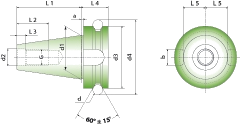
\includegraphics[width=.9\textwidth]{png/cone_1}
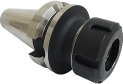
\includegraphics[width=.5\textwidth]{png/cone_2}

\textit{Attachement BT40 \cite{attachements}}
\end{center}
\end{minipage}\hfill
\begin{minipage}[c]{.3\linewidth}
\begin{center}
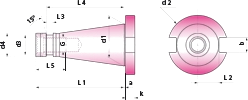
\includegraphics[width=.9\textwidth]{png/cone_3}
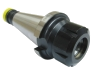
\includegraphics[width=.5\textwidth]{png/cone_4}

\textit{Attachement SA40 \cite{attachements}}
\end{center}
\end{minipage}\hfill
\begin{minipage}[c]{.3\linewidth}
\begin{center}
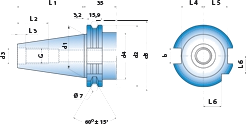
\includegraphics[width=.9\textwidth]{png/cone_5}
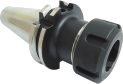
\includegraphics[width=.5\textwidth]{png/cone_6}

\textit{Attachement ISO40 \cite{attachements}}
\end{center}
\end{minipage}
\end{center}


\noindent\begin{minipage}[c]{.3\linewidth}
\begin{center}
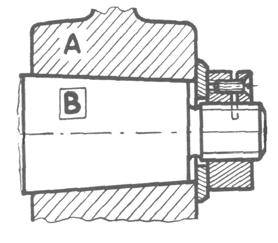
\includegraphics[width=.9\textwidth]{png/cone_7}
\end{center}
\end{minipage}\hfill
\begin{minipage}[c]{.3\linewidth}
\begin{center}
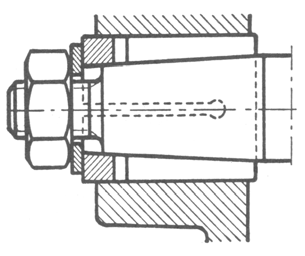
\includegraphics[width=.9\textwidth]{png/cone_8}
\end{center}
\end{minipage}\hfill
\begin{minipage}[c]{.3\linewidth}
\begin{center}
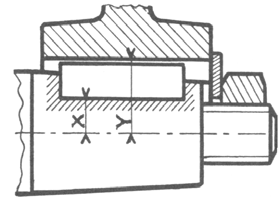
\includegraphics[width=.9\textwidth]{png/cone_9}
\end{center}
\end{minipage}

\vspace{.5cm}

\section{Réaliser le maintien en position entre pièces}
\subsection{Éléments filetés et taraudés -- Rappels}

\textbf{Pour plus d'information sur le tracé des éléments filetés, vous pouvez vous référez au chapitre 1.}


Les éléments filetés et taraudés regroupent les vis, les écrous, mais aussi les pièces fabriquées par tournage ou fraisage présentant un filet hélicoïdal. Bien qu'il existe des profils de vis trapézoïdaux ou ronds, le profil le plus utilisé est le \textbf{profil métrique ISO} (profil triangulaire).

\subsubsection{Désignation et représentation des vis}

\begin{center}
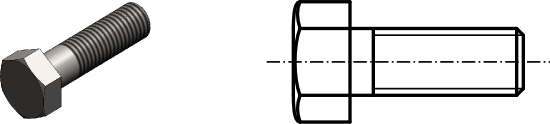
\includegraphics[width=.5\textwidth]{png/vis_rep}
\end{center}

Dans les nomenclatures, les vis sont désignées comme suit : 

\noindent\noindent\begin{minipage}[c]{.46\linewidth}
\begin{center}
NF ISO 4762 -- M10 x 30 -- 8.8
\end{center}
\end{minipage}\hfill
\noindent\begin{minipage}[c]{.46\linewidth}
\begin{itemize}
\item NF ISO 4762 : tête cylindrique à 6 pans creux
\item M : profil ISO (triangulaire)
\item 10 : diamètre nominal de la vis 
\item 30 : longueur filetée (en $mm$)
\item 8.8 : qualité de la vis ($8\times 100=800\; MPa$ : résistance minimale à la traction; $8\times 8 \time 10 = 640 \; MPa$ : limite minimale d'élasticité)
\end{itemize}
\end{minipage}

\vspace{.25cm}
Pour les filets ISO, le pas est directement donné en fonction du diamètre nominal (existence d'un pas gros (le plus courant) ou d'un pas fin).

%\subsubsection{Types de vis et formes de têtes}
%Une multitude de type de vis existent en fonction des besoins (vis d'assemblage, vis de pression) et des encombrements disponibles.
%
%En règle générale, les vis hexagonales et les vis cylindriques à embout hexagonal creux restent les plus utilisées. Ces dernières ont la possibilité de voir leurs têtes logées dans des lamages.
%\begin{center}
%\begin{tabular}{|m{7cm}|m{2.5cm}|m{2cm}|m{2.5cm}|m{2.5cm}|}
%\hline
%\textbf{Géométrie de la vis} & \textbf{Forme sous tête}  & \textbf{Forme tête} & & \textbf{Remarque}\\
%\hline \hline
%&&&& \\
%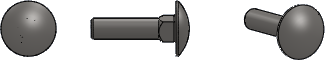
\includegraphics[width=6.5cm]{png/vis_1} &  & \textbf{B} -- Bombée & & Col carré\\
%\hline
%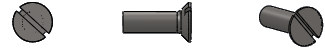
\includegraphics[width=6.5cm]{png/vis_2} &  \textbf{F} -- Fraisée &  & \textbf{S} -- Fendue& \\
%\hline
%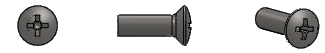
\includegraphics[width=6.5cm]{png/vis_3} & \textbf{F} -- Fraisée & \textbf{B} -- Bombée & \textbf{H} -- Cruciforme& \\
%\hline
%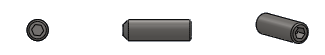
\includegraphics[width=6.5cm]{png/vis_4} & & & \textbf{HC} - hexagonal creux & Vis de pression\\
%\hline
%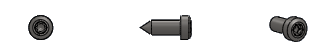
\includegraphics[width=6.5cm]{png/vis_5} & \textbf{C} -- Cylindrique & \textbf{B} - bombée & Torx & Auto foreuse \\
%\hline
%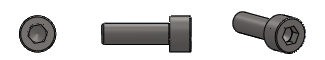
\includegraphics[width=6.5cm]{png/vis_6} & \textbf{C} -- Cylindrique & & \textbf{HC} -- hexagonal creux & \\
%\hline
%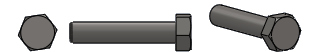
\includegraphics[width=6.5cm]{png/vis_7} & \textbf{H} -- Hexagonale & & & \\
%\hline
%\end{tabular}
%\end{center}
%
%
%
%
%\subsubsection{Écrous}
%\begin{center}
%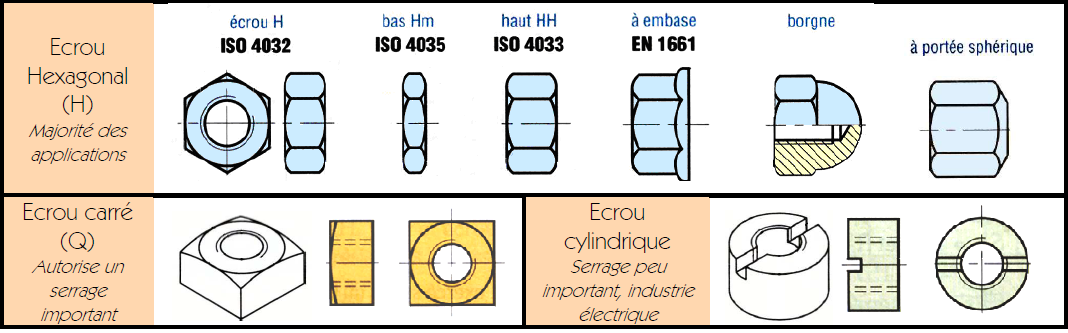
\includegraphics[width=.8\textwidth]{png/ecrous}
%\end{center}
%\subsubsection{Goujons}
%
%Un goujon est une tige cylindrique filetée aux deux extrémités. Il est vissé à fond de filetage dans une des pièces à assembler à l’aide d’une goujonneuse.
%Les goujons sont souvent utilisés pour assembler des pièces ne pouvant être traversées par des vis.
%lls sont également employés dans le cas de pièces en alliage léger, où le démontage trop fréquent de la vis risque de provoquer la détérioration des filets du trou taraudé.
%
%
%\begin{center}
%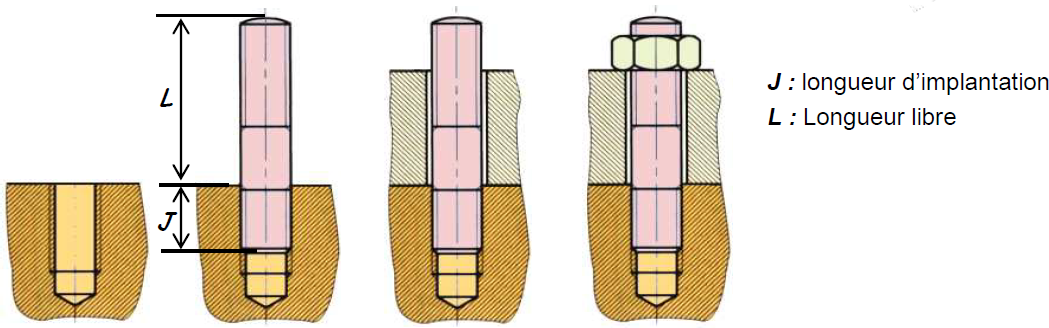
\includegraphics[width=.8\textwidth]{png/goujon}
%\end{center}
%
%Pour une vis l’implantation minimale J doit être au moins égale :
%\begin{itemize}
%\item $J \geq d$, diamètre nominal dans l’acier;
%\item $J \geq 1,5 \times d$, diamètre nominal dans la fonte, le cuivre;
%\item $J \geq 2 \times d$, diamètre nominal dans l’aluminium.
%\end{itemize}
%Pour un goujon l'implantation minimale J doit être au moins égale :	 
%\begin{itemize}
%\item $J \geq 1,5 \times d$, diamètre nominal dans l’acier;
%\item $J \geq 2 \times d$, diamètre nominal dans un métal tendre.
%\end{itemize}
%
%
%\subsubsection{Technologie des éléments filetés}
%\paragraph*{Matériaux}
%\begin{center}
%\begin{tabular}{|c|c|c|c|c|}
%\multicolumn{5}{c}{\textbf{Matériaux des vis}} \\ \hline
%Catégorie & Matière & État & $\quad Rm \quad $ & $\quad Re \quad $ \\ \hline
%Acier non traité & $2\; 235$ & -- & 340 & 235 \\ \hline
%Acier traité & $25\;Cr\;Mo\; 4$ & Trempé revenu & 930 & 785 \\ \hline
%Acier inoxydable & $X\; 30 \;Cr\;Ni\; 18-10$ & Trempé revenu & 900 & 750 \\ \hline
%\end{tabular}
%\end{center}
%
%\paragraph*{Fabrication}
%Le processus de fabrication des vis est généralement proche de cela : 
%\begin{itemize}
%\item laminage : obtention de rouleau de fil (le diamètre du fil pouvant aller jusqu'à plusieurs dizaines de $mm$);
%\item redressage afin de redresser le rouleau en tige;
%\item découpage des tronçons;
%\item forgeage à froid (avec plusieurs matrices) de la tête de vis;
%\item chanfreinage du bout de vis;
%\item roulage du filetage;
%\item traitement thermique.
%\end{itemize}
%
%
%Lorsqu'il s'agit de fabriquer des arbres filetés ou des moyeux taraudés, il est possible d'utiliser des procédés de filetage (tournage) ou de taraudage (tournage ou fraisage). 
%
%En tournage, lorsqu'un outil à fileter est utilisé, un gorge doit être réalisée avant un épaulement. Cette dernière empêche ainsi l'outil de de butter contre un plan. 
%
%Lors de l'utilisation d'un taraud sur un centre d'usinage, la broche se doit d'être asservie. En effet, une mauvaise synchronisation des axes provoquerait une casse du filet. 
%
%\noindent\begin{minipage}[c]{.3\linewidth}
%\begin{center}
%\includegraphics[width=.8\textwidth]{png/taraudage_lisse}
%\end{center}
%
%\noindent\textit{Taraudage dans un trou borgne : le trou de perçage réaliser grâce à un foret est plus profond que la partie taraudée.}
%\end{minipage}\hfill
%\begin{minipage}[c]{.3\linewidth}
%\begin{center}
%\includegraphics[width=.8\textwidth]{png/taraudage_epaul}
%\end{center}
%
%\noindent\textit{Taraudage terminant par un épaulement : ou bien le taraudage s'arrête bien avant l'épaulement, ou bien on prévoit une gorge de dégagement.}
%\end{minipage}\hfill
%\begin{minipage}[c]{.3\linewidth}
%\begin{center}
%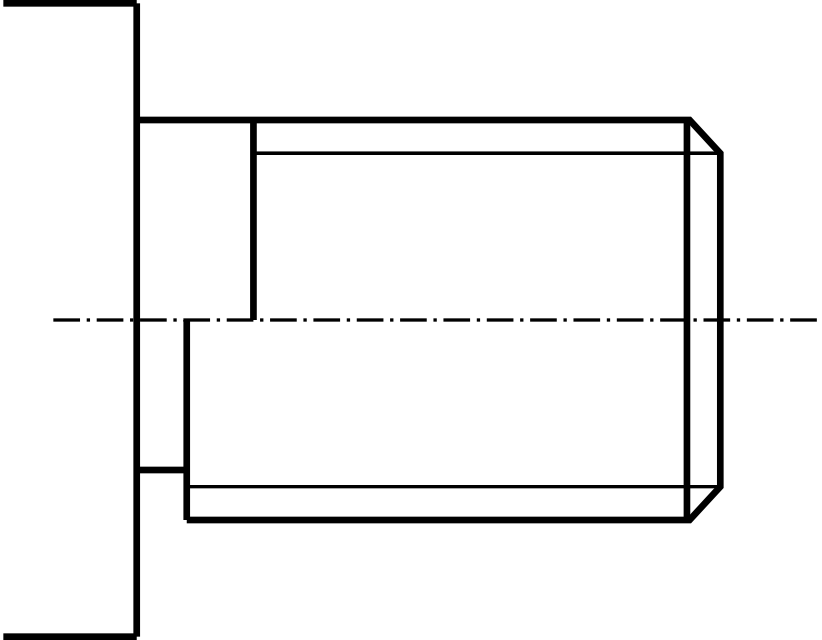
\includegraphics[width=.8\textwidth]{png/epaulement}
%\end{center}
%
%\noindent\textit{Filetage terminant par un épaulement : préférer la solution avec une gorge en fin de filetage.}
%\end{minipage}
%
%
%\paragraph*{Classe de qualité}
%La classe de qualité de vis est généralement marquée sur la tête. Elle indique le comportement de la vis lorsqu'elle est soumise à des efforts axiaux. Elle est composée de deux chiffres séparés par un point : $a.b$.
%
%$a\times 100$ donne la limite à la rupture de la vis.
%
%$a\times b\times 10$ donne la limite à l'élasticité de la vis. 
%
%Ces valeurs sont déterminées par des essais de traction. 
%
%\textbf{Attention à ne pas solliciter les vis en cisaillement. Il ne faut donc pas utiliser les vis pour assurer une mise en position.}
%
%\begin{center}
%\begin{tabular}{|l|c|c|c|c|c|c|c|c|c|c|}
%\hline
%Classe de résistance & 
%$3.6$ & $4.6$ & $4.8$ & $5.6$ & $5.8$ & $6.8$ & $8.8$ & $9.8$ & $10.9$ & $12.9$ \\
%\hline 
%Limite élastique ($MPa$) & 180 & 240 & 320 & 300 & 400 & 480 & 640 & 720 & 900 & 1 080 \\
%\hline
%Limite à la rupture  ($MPa$) & 330 & 400 & 420 & 500 & 520 & 600 & 800 & 900 & 1 040 & 1 220 \\
%\hline
%\end{tabular}
%\end{center}
%
%\subsubsection{Dimensionnement des assemblages filetés}

\subsubsection{Conception des assemblages vissés}
Maintien en position lors de la mise en position par appui plan prépondérant et centrage court :

\begin{center}
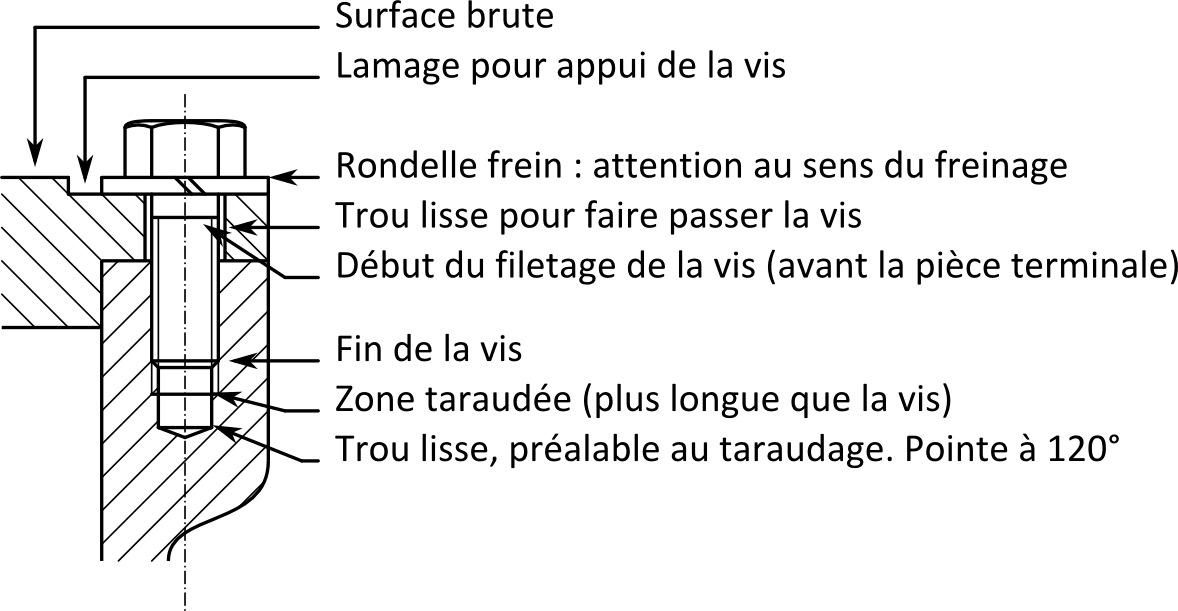
\includegraphics[width=.8\textwidth]{png/Fig30_1}
\end{center}

\noindent\begin{minipage}[c]{.3\linewidth}
\begin{center}
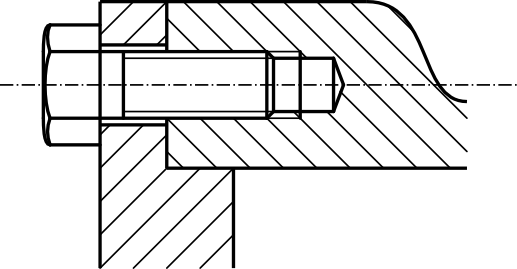
\includegraphics[width=.9\textwidth]{png/Fig30_2}

\textbf{Assemblage avec vis Hexagonale}
\end{center}
\end{minipage}\hfill
\begin{minipage}[c]{.3\linewidth}
\begin{center}
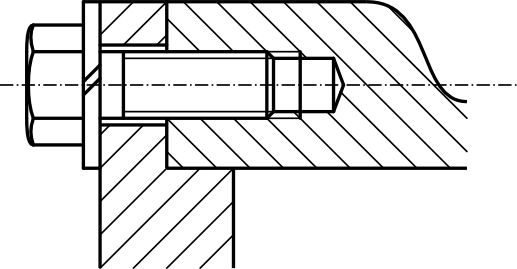
\includegraphics[width=.9\textwidth]{png/Fig30_3}

\textbf{Assemblage avec vis Hexagonale et rondelle frein}
\end{center}
\end{minipage}\hfill
\begin{minipage}[c]{.3\linewidth}
\begin{center}
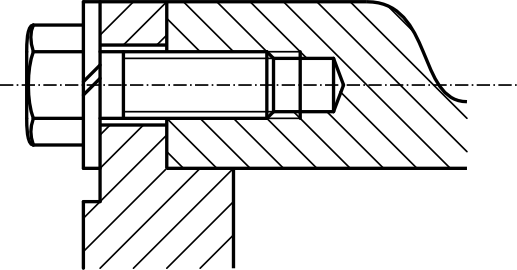
\includegraphics[width=.9\textwidth]{png/Fig30_6}

\textbf{Assemblage avec vis Hexagonale, rondelle frein et lamage}
\end{center}
\end{minipage}

\vspace{.5cm}

\noindent\hspace{.15\textwidth}\begin{minipage}[c]{.3\linewidth}
\begin{center}
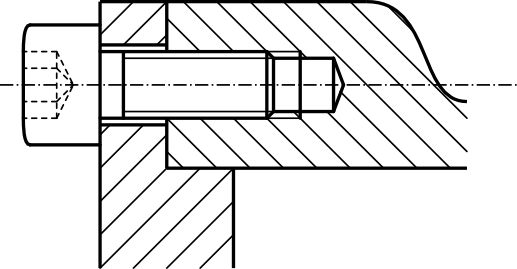
\includegraphics[width=.9\textwidth]{png/Fig30_4}

\textbf{Assemblage avec vis CHC}
\end{center}
\end{minipage}\hfill
\begin{minipage}[c]{.3\linewidth}
\begin{center}
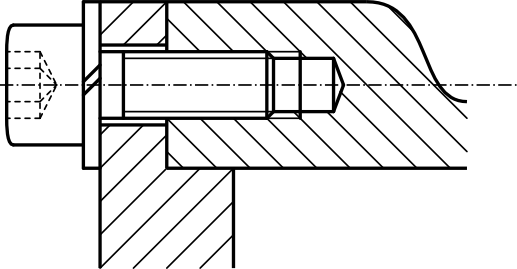
\includegraphics[width=.9\textwidth]{png/Fig30_5}

\textbf{Assemblage avec vis CHC et rondelle frein}
\end{center}
\end{minipage}\hspace{.15\textwidth}


\vspace{.5cm}

Maintien en position lors de la mise en position par centrage long et appui ponctuel :
\begin{center}
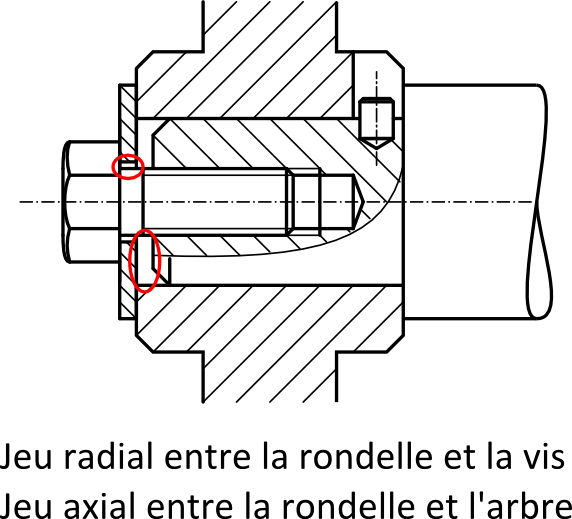
\includegraphics[width=.4\textwidth]{png/Fig31}

\end{center}

\vspace{.5cm}

Suivant la tête de vis utilisée et suivant la provenance du brut, il est possible de donner des formes différentes à la zone de contact entre la tête de vis et le support. 

\begin{center}
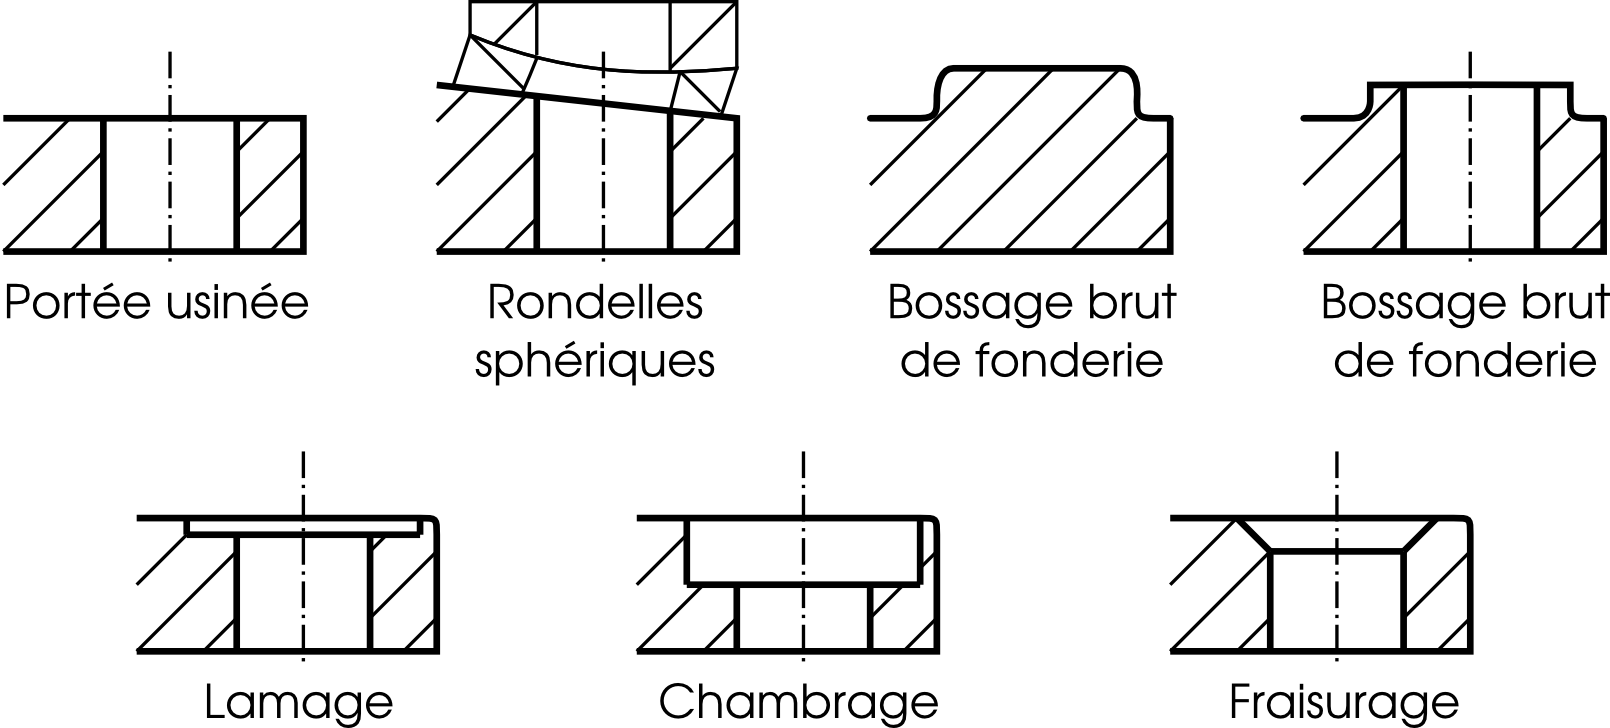
\includegraphics[width=.7\textwidth]{png/portees}
\end{center}



\subsubsection{Conception des assemblages boulonnés}

On parle d'assemblage boulonné lorsque au moins deux pièces sont maintenues en position par \textbf{une vis et un écrou}. Dans ce cas, les perçages des pièces sont \textbf{lisses}.

\begin{center}
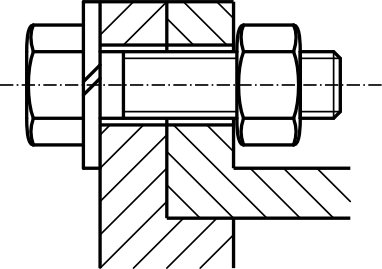
\includegraphics[width=.3\textwidth]{png/Fig30_7}

\end{center}


\subsection{Rivetage}
\noindent\begin{minipage}[c]{.46\linewidth}
Le rivetage est un procédé utilisé pour assembler des tôles de matériaux différentes et d'épaisseurs différentes. Ce procédé est très utilisé dans l'aéronautique pour assembler les panneaux constituants le fuselage des appareils. 

Pour riveter des tôles, il est nécessaire de les pré-percer. On fait alors passer une tige métallique à tête ronde. L'autre extrémité de la tige est aplatie afin de rendre les tôles solidaires l'une de l'autre. 
\end{minipage}\hfill
\begin{minipage}[c]{.46\linewidth}
\begin{center}
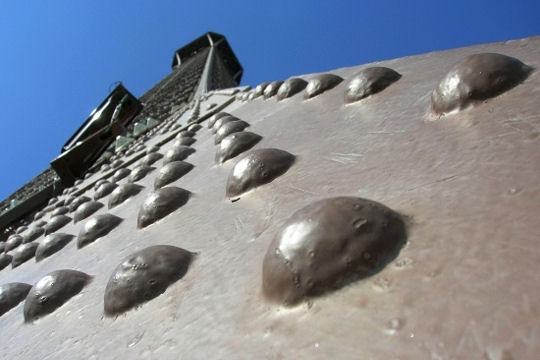
\includegraphics[width=.8\textwidth]{png/rivets}

\textit{Assemblage rivetés sur la Tour Eiffel \cite{rivets}}
\end{center}
\end{minipage}
\subsection{Soudage}

Le soudage permet d'assembler deux pièces par fusion locale de chacune des pièces avec présence ou non d'un métal d'apport. Il existe une multitude de procédés de soudage. Nous n'en présenterons que deux de manière succincte. 

Tout d'abord, le MIG (metal inert gaz) est un procédé de soudage à l'arc au cours duquel la zone de fusion est protégée par un gaz inerte. Un arc électrique est créé entre la pièce et une électrode consommable. Du gaz (argon, hélium, $CO_2$ ou mélange) est projeté autour de l'électrode par une buse. Ce procédé permet d'assembler des métaux ferreux ou non ferreux, sur une épaisseur plus ou moins grande. La relative facilité de mise en œuvre de ce procédé le rend facilement automatisable.

Le TIG (tungsten inert gaz) est un procédé proche du précédent. Dans ce cas, l'électrode est en tungstène; elle est non consommable. Le matériau d'apport est mis à disposition par une autre baguette. Le TIG permet de souder des épaisseurs fines avec une excellente qualité.

Lors de la conception de pièces qui doivent être mécano soudées, il est nécessaire de préparer les bords des tôles à souder. Cela fera l'objet d'un cours en PT. 


\subsection{Colles}
Même si le procédé de collage est largement utilisé dans l'industrie, l'utilisation de ce procédé est à proscrire lors de la conception des mécanismes en PTSI et en PT. 

\section{Transmettre la puissance}

Lorsqu'il s'agit de transmettre de la puissance entre des pièces mécaniques, il est possible d'utiliser des éléments technologiques supplémentaires afin de mieux résister aux efforts. 

%\subsection{Goupilles}
\subsection{Transmission par clavettes}

\subsubsection{Profil des clavettes}
La plupart du temps, les clavettes servent d'une part à assurer la mise en position lors d'une liaison encastrement démontable. D'autre part, elle permette d'assurer la transmission de puissance entre, par exemple, un arbre et un pignon ou une poulie.

Elles sont désignées ainsi :

\noindent\begin{minipage}[c]{.4\linewidth}
\begin{center}
Clavette parallèle, forme A, a x b x l
\end{center}

\end{minipage}\hfill
\begin{minipage}[c]{.4\linewidth}
\begin{center}
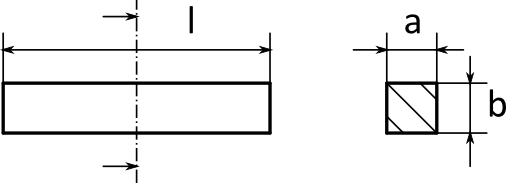
\includegraphics[width=.9\textwidth]{png/clavette}
\end{center}
\end{minipage}


\noindent\begin{minipage}[c]{.22\linewidth}
\begin{center}
\includegraphics[width=.6\textwidth]{png/clavettea}

\textbf{Clavette de type A}
\end{center}
\end{minipage}\hfill
\begin{minipage}[c]{.22\linewidth}
\begin{center}
\includegraphics[width=.6\textwidth]{png/clavetteb}

\textbf{Clavette de type B}
\end{center}
\end{minipage}\hfill
\begin{minipage}[c]{.22\linewidth}
\begin{center}
\includegraphics[width=.6\textwidth]{png/clavettec}

\textbf{Clavette de type C}
\end{center}
\end{minipage}\hfill
\begin{minipage}[c]{.22\linewidth}
\begin{center}
\includegraphics[width=.6\textwidth]{png/clavetted}

\textbf{Clavette disque}
\end{center}
\end{minipage}\hfill


\subsubsection{Profil des arbres}


\begin{center}
\begin{tabular}{m{2cm}m{5cm}m{2cm}m{5cm}}
\multicolumn{4}{c}{\textbf{Arbre usiné à la fraise 2 tailles}} \\
\includegraphics[width=2cm]{png/rainure1_3d}&
\includegraphics[width=5cm]{png/rainure1}&
\includegraphics[width=2cm]{png/rainure2_3d} &
\includegraphics[width=5cm]{png/rainure2}\\
\end{tabular}
\end{center}

\begin{center}
\begin{tabular}{m{2cm}m{5cm}m{2cm}m{5cm}}
\multicolumn{4}{c}{\textbf{Arbre usiné à la fraise 3 tailles}} \\
\includegraphics[width=2cm]{png/rainure3_3d}&
\includegraphics[width=5cm]{png/rainure3}&
\includegraphics[width=2cm]{png/rainure4_3d}&
\includegraphics[width=5cm]{png/rainure4}
\end{tabular}
\end{center}

%\subsubsection{Profil des moyeux}

\subsubsection{Conception des assemblages clavetés}

\noindent\begin{minipage}[c]{.45\linewidth}
 \begin{center}
  \includegraphics[height=5cm]{png/Fig2}
%\textbf{Fig 2 -- Réf 1, 2, 5, 9, 14, 15}
 \end{center}

\begin{itemize}
\item Arrêt en rotation par clavette disque 
\item Pour couple peu importants
\item Rainure debouchante -- obligatoire sur le moyeu.
\end{itemize}
 \end{minipage} \hfill
\noindent\begin{minipage}[c]{.45\linewidth}
 \begin{center}
  \includegraphics[height=5cm]{png/Fig4}
%\textbf{Fig 4 -- Réf 1, 2, 6, 9, 17, 18}
\end{center}

\begin{itemize}
\item Arrêt en rotation par clavette parallèle
\item Couples importants
\item Freinage par obstacle
\item Rainure débouchante sur le moyeu
\end{itemize}

\end{minipage} 


\noindent\begin{minipage}[c]{.45\linewidth}

 
\end{minipage} \hfill
\noindent\begin{minipage}[c]{.45\linewidth}
 
\end{minipage} 

\noindent\begin{minipage}[c]{.45\linewidth}
 \begin{center}
  \includegraphics[height=5cm]{png/Fig5}

%\textbf{Fig 5 -- Réf 1, 2, 6, 9, 17, 18}

 \end{center}



\begin{itemize}
\item Arrêt en rotation par clavette parallèle représentée de face
\item Freinage par adhérence rondelle à dents
\end{itemize}
 
\end{minipage} \hfill
\noindent\begin{minipage}[c]{.45\linewidth}
 \begin{center}
  \includegraphics[height=5cm]{png/Fig6}

%\textbf{Fig 6 -- Réf 1, 2, 6, 9, 17, 18}

 \end{center}


\begin{itemize}
\item Même solution
\item Freinage avec un écrou «~Nylstop~»
\end{itemize}
 
\end{minipage} 


\noindent\begin{minipage}[c]{.45\linewidth}
 \begin{center}
  \includegraphics[height=5cm]{png/Fig7}

%\textbf{Fig 7 -- Réf 1, 2, 6, 9, 17, 18}
 \end{center}


\begin{itemize}
\item Même solution
\item Freinage par obstacle avec écrou SKF et rondelle à languette
\end{itemize}
 
\end{minipage} 

\subsubsection{Dimensionnement des assemblages clavettés}


%\begin{minipage}[c]{.55\linewidth}
On calcule les clavettes au matage (critère
lié à la pression de contact admissible).

Un couple de moment $Ct$ est transmis par la clavette 34 du pignon 30 à l'arbre
35. On souhaite déterminer la longueur de clavette minimale pour éviter le
phénomène de matage qui représente un écrasement permanent de la surface dû à
une trop forte pression de contact. 
%\end{minipage} \hfill
%\begin{minipage}[c]{.4\linewidth}
%\begin{center}
% \includegraphics[width=.9\textwidth]{png/im1}
%\end{center}
%\end{minipage} 

\paragraph*{Hypothèse de calcul et paramètres géométriques}
On suppose que l'intégralité du couple est transmis par la clavette seule et
non par l'ajustement arbre/alésage.

Le contact est supposé plan et la pression de contact uniforme.

\paragraph*{Données géométriques}

%\begin{minipage}[c]{.55\linewidth}
\begin{itemize}
 \item La zone de contact, sur la clavette, est un rectangle de longueur $L$ et
de hauteur $h$  (à déterminer avec un tableau de normes.
\item Les dimensions ($s\times s$) du chanfrein de la clavette sont souvent négligés
(et jamais représentés). Nous considérons que $s=0$. 
\item Aire de la surface de contact : $A=L \times h$.
\item Hauteur de clavette en prise dans le moyeu : $h=b-(d-j)$.
\item La valeur de $d$ est toujours connue et impose les valeurs $a$, $b$, $j$
donc celle de $h$.
\end{itemize}
%\end{minipage} \hfill
%\begin{minipage}[c]{.4\linewidth}
%\begin{center}
% \includegraphics[width=.8\textwidth]{png/im2}
%\includegraphics[width=.7\textwidth]{png/im3}
%\end{center}
%\end{minipage} 

\paragraph*{Détermination de la pression de contact}
\begin{itemize}
 \item La pression étant uniforme, $p=F/A$.
\item Couple transmis : $C=F\times (d/S+e)$ (Nous considérons que $e=0$, ce qui
majore $p$).
\end{itemize}

%\begin{center}
% \includegraphics[width=.8\textwidth]{png/im4}
%\end{center}

Avec l'hypothèse de répartition de pression uniforme, on a : 
$$
p = \dfrac{C}{\dfrac{d}{2}Lh}
$$

\paragraph*{Détermination de la longueur utile de la clavette}

Pour vérifier la résistance au matage d'une clavette, il faut vérifier que la
pression de contact reste inférieure à la pression admissible. Les valeurs de
pression admissibles avant matage dépendent principalement des propriétés
mécaniques du matériau utilisé et des conditions de fonctionnement. Elles sont
données dans les normes ou documents constructeurs.


\begin{center}
 \begin{tabular}{|c|c|c|c|}
\hline
Montage & Conditions de fonctionnement & Clavettes & Cannelures \\
 & & (Acier : $Rr = 600\;MPa$) & (Acier $Rr = 1000 MPa$) \\
\hline
\multirow{3}*{Glissant en charge}& Avec à coups ou vibrations & de 0,5 à 2 MPa &
de 5 à 10 MPa \\
\cline{2-4}
& Cas général & de 2 à 6 MPa & de 10 à 20 MPa \\
\cline{2-4}
& Charge et vitesse constante & de 6 à 10 MPa & de 20 à 30 MPa \\
\hline
\multirow{3}*{Fixe}
& Avec à coups ou vibrations & de 10 à 20 MPa & de 30 à 60 MPa \\
\cline{2-4}
& Cas général & de 20 à 40 MPa & de 60 à 120 MPa \\
\cline{2-4}
& Charge et vitesse constante & de 40 à 90 MPa & de 120 à 180 MPa \\
\hline
 \end{tabular}
\end{center}

Nous devons vérifier que : $p<p_{admissible}$, soit : 
$$
\dfrac{C}{\dfrac{d}{2}Lh}\leq p_{admissible}
$$

Cette inéquation permet de calculer la longueur «~utile~» $L$ de la clavette,
(il faut ajouter les arrondis de rayon $a/2$ suivant la forme $A$ ou $C$ de la
clavette). On évitera : $l>1,8d$.

\paragraph*{Exemple de calcul}
\begin{itemize}
 \item Couple à transmettre : $C=60 Nm$
\item Diamètre de l'arbre : $d=40 mm$
\item La norme indique donc : $a=12$, $b=8$, $j=25$
\end{itemize}

Il s'agit d'un assemblage fixe (pas de guidage de translation) avec un risque
de vibration (engrenage à denture droite) la pression admissible retenue est
$p_{admissible}=20 \; MPa$.

Il est demandé de déterminer complètement les dimensions de la clavette de
forme $C$ permettant de transmettre le couple demandé sans que la surface de
contact de la clavette soit matée. 













\subsection{Cannelures}
 \begin{center}
  \includegraphics[height=5cm]{png/Fig8}

%\textbf{Fig 8 -- Réf 1, 2, 7, 9, 14, 16}
 \end{center}

\begin{itemize}
\item Arrêt en rotation par cannelures
\item Pour couples très importants, avec chocs éventuels
\item Remarquer le freinage par obstacle de la vis
\end{itemize}

\subsection{Autres dispositifs d'arrêts par obstacles}

\noindent\begin{minipage}[c]{.45\linewidth}
 \begin{center}
  \includegraphics[height=5cm]{png/Fig1}
%\textbf{Fig 1 -- Réf 1, 2, 3, 9, 14, 16}
\end{center}

\begin{itemize}
\item Arrêt en rotation par pion cylindrique
\item Pour couples faibles et sans choc
\item Remarquer le freinage de la vis
\end{itemize}
\end{minipage} \hfill
\noindent\begin{minipage}[c]{.45\linewidth}
 \begin{center}
  \includegraphics[height=5cm]{png/Fig3}
%\textbf{Fig 3 -- Réf 1, 2, 4, 9, 14, 15}
 \end{center}

\begin{itemize}
\item Arrêt en rotation par goupille «~entre cuir et chair~»
\item Couples peu importants
\item Perçage du logement de goupille lors du montage
\end{itemize}
\end{minipage} 

\noindent\begin{minipage}[c]{.9\linewidth}
\end{minipage} 

\noindent\begin{minipage}[c]{.45\linewidth}
 \begin{center}
  \includegraphics[height=5cm]{png/Fig11}
%\textbf{Fig 11 -- Réf 1, 2, ...}
 \end{center}

\begin{itemize}
\item Centrage et maintien en position par adhérence efficace avec un manchon
«~Ringblock série 1300~»
\item Réglage possible de la position angulaire et axiale avec serrage
\item Utilisé sur arbre lisse
\end{itemize}
\end{minipage} \hfill
\noindent\begin{minipage}[c]{.45\linewidth}
 \begin{center}
  \includegraphics[height=5cm]{png/Fig12}
%\textbf{Fig 10 -- Réf 1, 2...}
 \end{center}

\begin{itemize}
\item Centrage et maintien en position par adhérence efficace avec un manchon
«~Trantorque~»
\item Réglage possible de la position angulaire et axiale avant serrage
\item Utilisé sur arbre lisse
\end{itemize}
\end{minipage} 

\noindent\begin{minipage}[c]{.45\linewidth}
 \begin{center}
  \includegraphics[height=5cm]{png/Fig12Bis}
%\textbf{Fig 12 -- Réf 1, 2, 9, ...}
 \end{center}

\begin{itemize}
\item Maintien en position par adhérence avec des éléments «~Ringblock série
1060~» empilés 
\item Moins encombrants, moins chers mais transmettent un couple moins important
\item Un centrage est conseillé
\end{itemize}
\end{minipage} \hfill
\noindent\begin{minipage}[c]{.45\linewidth}
 \begin{center}
  \includegraphics[height=5cm]{png/Fig13}
%\textbf{Fig 13 -- Réf 1, 2, 9, 19}
 \end{center}

\begin{itemize}
\item Maintien en rotation et en translation par adhérence avec un empilage de
rondelles élastiques «~Ringspann~»
\end{itemize} 
\end{minipage} 

\noindent\begin{minipage}[c]{.45\linewidth}
 \begin{center}
  \includegraphics[height=4cm]{png/Fig14}
%\textbf{Fig 14 -- Réf 1, 2, 20}
 \end{center}

\begin{itemize}
\item Centrage et maintien en position par adhérence efficace avec des éléments
«~Tollock~»
\item Réglage possible de la position angulaire et axiale avec serrage
\item Utilisé sur arbre lisse
\end{itemize} 
\end{minipage} \hfill
\noindent\begin{minipage}[c]{.45\linewidth}
 \begin{center}
  \includegraphics[width=.9\textwidth]{png/Fig9}
%\textbf{Fig 9 -- Réf 1, 2, 10, 11}
 \end{center}

\begin{itemize}
\item Arrêt en rotation et translation par goupille transversale
\item Mise en position latérale peu précise.
\item Ici utilisation de goupilles élastiques
\end{itemize}
\end{minipage} 



\section{Assurer l'étanchéité}
Plusieurs solutions permettent d'assurer l'étanchéité d'un mécanisme. Nous nous intéressons ici aux solutions d'étanchéité statique (par "opposition" aux solutions d'étanchéité dynamique).

\noindent\begin{minipage}[c]{.3\linewidth}
\begin{center}
\includegraphics[width=.9\textwidth]{png/papier}

\textit{Joint papier \cite{papier}}
\end{center}
\end{minipage}\hfill
\begin{minipage}[c]{.3\linewidth}
\begin{center}
\includegraphics[width=.9\textwidth]{png/torique}

\textit{Joint torique \cite{torique}}
\end{center}
\end{minipage}\hfill
\begin{minipage}[c]{.3\linewidth}
\begin{center}
\includegraphics[width=.9\textwidth]{png/culasse}

\textit{Joint de culasse \cite{culasse}}
\end{center}
\end{minipage}


\section{Assurer la fiabilité}
Les chocs, les vibrations répétées, les variations de température auxquels sont soumis les assemblages par
éléments filetés, peuvent très rapidement entraîner leur desserrage (perte de la pression de contact entre
filets de la vis et de l'écrou).


\subsection{Écrou freiné}
\begin{center}
\includegraphics[width=.8\textwidth]{png/ecrous_2}
\end{center}

\begin{center}
\includegraphics[width=.8\textwidth]{png/ecrous_3}
\end{center}

\subsection{Rondelles}

\begin{center}
\includegraphics[width=.8\textwidth]{png/rondelles}
\end{center}

\begin{thebibliography}{2}
\bibitem{ls}{\url{http://www.hellopro.fr/images/produit-2/2/4/9/motoreducteur-a-sortie-axiale-207942.jpg}}
\bibitem{sew}{\url{http://www.cnr-cmao.ens-cachan.fr/fiches_dossiers/motoreducteur_sew_r17_DT.php?t=13}}
\bibitem{poclain}{\url{http://www.cnr-cmao.ens-cachan.fr/}}
\bibitem{poclain}{Fabrication de vis : \url{http://www.youtube.com/watch?v=7ORomNNCSUQ}}
\bibitem{attachements}{http://www.gbmo.eu/attachement-pour-le-fraisage.html}
\bibitem{attachements_2}{http://www.maritool.com/images/HSK50A-ER32-COLLET-CHUCK-1.jpg}
\bibitem{mc}{Supports de cours de Maryline Carrez, Lycée Jules Haag, Besançon}
\bibitem{rivets}{\url{http://www.linternaute.com/paris/magazine/photo/la-tour-eiffel-dans-tous-ses-etats/image/rivets-d-eiffel-441056.jpg}}
\bibitem{pf}{Supports de cours de Philippe Fichou, Lycée Vauban, Brest \url{http://philippe.fichou.pagesperso-orange.fr/documents/liaisoncomplete2003.pdf}}
\bibitem{torique}{\url{http://www.via-industry.com/rep_images/client/magicap/jointstoriques.jpg}}
\bibitem{papier}{\url{http://membres.multimania.fr/solokoy/img/Joints\%20papier.jpg}}
\bibitem{culasse}{\url{http://www.vlvautoparts.com/vlvautoparts_images/produits/12.4726.jpg}}
\end{thebibliography}

\end{document}